%
% Conclusion - The Vision of the Quantum Internet
%

\famousquote{When something is important enough, you do it even if the odds are not in your favour.}{Elon Musk}
\newline

\famousquote{Be nice to nerds. Chances are you'll end up working for one.}{Bill Gates}
\newline

\famousquote{We are just an advanced breed of monkeys on a minor planet of a very average star. But we can understand the Universe. That makes us something very special.}{Stephen Hawking}
\newline

\section{Conclusion -- The vision of the quantum internet} \label{sec:vision_quant} \index{Vision of the quantum internet}\index{Conclusion}

\famousquote{We will either go down as the world's greatest statesmen, or its greatest villains}{Hermann G{\" o}ring}
\newline

\comment{Include ref} %Fig.~\ref{fig:integrated_services_overview}

\dropcap{Q}{uantum} technologies, particularly quantum computing, will truly revolutionise countless industries. With early demonstrations of key quantum technologies -- such as QKD, long distance quantum teleportation, and quantum computing -- becoming a reality, it is of utmost importance that networking protocols be pursued now.

We have presented an early formulation and analysis of quantum networking protocols with the vision of enabling a future quantum internet, where quantum resources can be shared and communicated in much the same way as is presently done with digital assets. Whilst it's hard to foresee exactly how future quantum networks will be implemented, as there are many unknowns, many of the central ideas presented here will be applicable across architectures and implementations on an ad hoc basis.

There are a number of schools of thought one might subscribe to when quantum networking. One might demand perfect data integrity and best-case network performance. But that would come at the expense of necessitating an all-powerful central authority to oversee all communications, ensuring that scheduling was absolutely perfect -- a potentially very challenging optimisation problem. Or one might tolerate lost data packets or suboptimal performance, at the expense of limiting applicability, but with the benefit of improved flexibility and reconfigurability. Or maybe some arbitrary compromise between different metrics and attributes is best. These are open questions that needn't have concrete, one-size-fits-all answers. They certainly needn't be answered right now.

The QTCP framework we presented is sufficiently flexible and extensible that these questions can be answered and enforced independently by different subnets, depending on their individual characteristics and requirements, in much the same way that every organisation connected to the classical internet today is free to structure their own LAN as they please, enforcing their own internal network policies.

The quantum internet will allow quantum computation to become distributed, not just outsourced. In the same way that many present-day classical algorithms are heavily parallelised and distributed across large clusters, CUDA cores\index{CUDA}, or even across the internet itself (e.g the SETI project\index{SETI project}), quantum networks will allow the distribution of quantum computation across many nodes, either in parallel, in series, or in a modularised fashion. This will be pivotal to achieving scalability. Keeping in mind that the classical-equivalent power of a quantum computer may grow exponentially with the number of qubits, it is highly desirable to squeeze out every last available qubit for our computations -- every qubit is worth more than the last!

Combined with recent advances in homomorphic encryption and blind quantum computation, commercial models for the distribution of quantum computation will emerge, allowing computational power to be outsourced, with both client and server confident in the security of their data and proprietary algorithms. This is a notion that is challenging on classical computers, but will be of utmost importance in quantum computing, where it is expected sensitive or valuable data and algorithms will often be at stake.

From the security perspective, the global quantum internet will enable an international QKD communications network with perfect secrecy, guaranteed to be information-theoretically secure by the laws of physics. This will be of immense economic and strategic benefit to commercial enterprises, governments, and individuals. Classical cryptography is already a multi-billion dollar industry worldwide. Quantum cryptography will supersede it, and be of especial importance in the era of quantum computers, which compromise some essential classical cryptographic protocols, such as RSA, which forms the basis of most current internet encryption, digital signatures, and the Blockchain/Bitcoin protocols. Not only is quantum cryptography being pursued optically, but even credit cards with embedded quantum circuitry are being actively developed to prevent fraud. Inevitably, this will require the communication between bank automats and servers to be mediated by a quantum network.

Already, off-the-shelf QKD systems are available as commodity items, from vendors such as MagiQ\index{MagiQ} and ID Quantique\index{ID Quantique}, which may be simply interconnected via an optical fibre link, thereby implementing end-to-end quantum cryptography in a modularised fashion. This is of a similar flavour to, and first technological step towards, modularised quantum computing, which would greatly enhance the economic viability and scalability of general purpose quantum computing by paving the way for the mass production of elementary interconnectable modules as commodity items.

We have focussed our attention thus far on the application of quantum networking to quantum information processing applications, such as quantum computing and quantum cryptography. However, with plug-and-play quantum resources available over a network, one might envisage far greater applicability than just these.

Of particular interest are the implications of quantum networking to basic science research. Presently, experimental quantum physics research is limited to well-resourced labs with access to state of the art equipment. With the ability to license these assets over a network, and dynamically interconnect them on an ad hoc basis, the ability to construct all manner of quantum experiments could be extended to all. An undergraduate laboratory would now have the ability to approach a host to politely borrow their state engineering technologies, send it to another with the ability to perform some evolution to that system, and to yet another to perform measurement and analysis of the output -- all from an undergrad lab equipped with nothing more than desktop PCs. This has broad implications for basic science research, opening it up to aspiring researchers across the globe, regardless of their direct access to cutting-edge tools. This will greatly expand the intellectual base for conducting quantum experimentation to the entire global scientific community, decimating the scientific monopolies controlled by a handful of world-leading, highly-resourced experimental teams.

The reality is that we are only just beginning to understand the full potential for quantum technologies, and as we learn more we will inevitably find new uses for networking them. The full potential of digital electronics was never fully realised (or anticipated) until the emergence of the internet. It is to be expected the same will hold in the quantum era, an era only in its inception.

Large-scale quantum computing may still seem a formidable, and somewhat long-term challenge. But it isn't likely to remain so. Once we have mastered the technological art of preparing qubits and implementing high-fidelity entangling operations between them, it's just a matter of sitting back and watching Gordon Moore\index{Moore's Law} perform his witchcraft, and scalability of quantum technology, and its rapid market-driven reduction in cost, will quickly ensue. The quantum internet will drive this rapid development by expanding both the supply and demand for access to this technology, and through unification of computational resources allow them to massively enhance their collective computational power, beyond their individual capabilities.

It is essential for the adoption and development of quantum technology, that quantum networking infrastructure be sufficiently well developed that it is ready to be deployed the minute the first useful, post-classical hardware becomes available. The proliferation of the defining technology of the 21st century depends upon it.

\begin{figure*}[!htbp]
	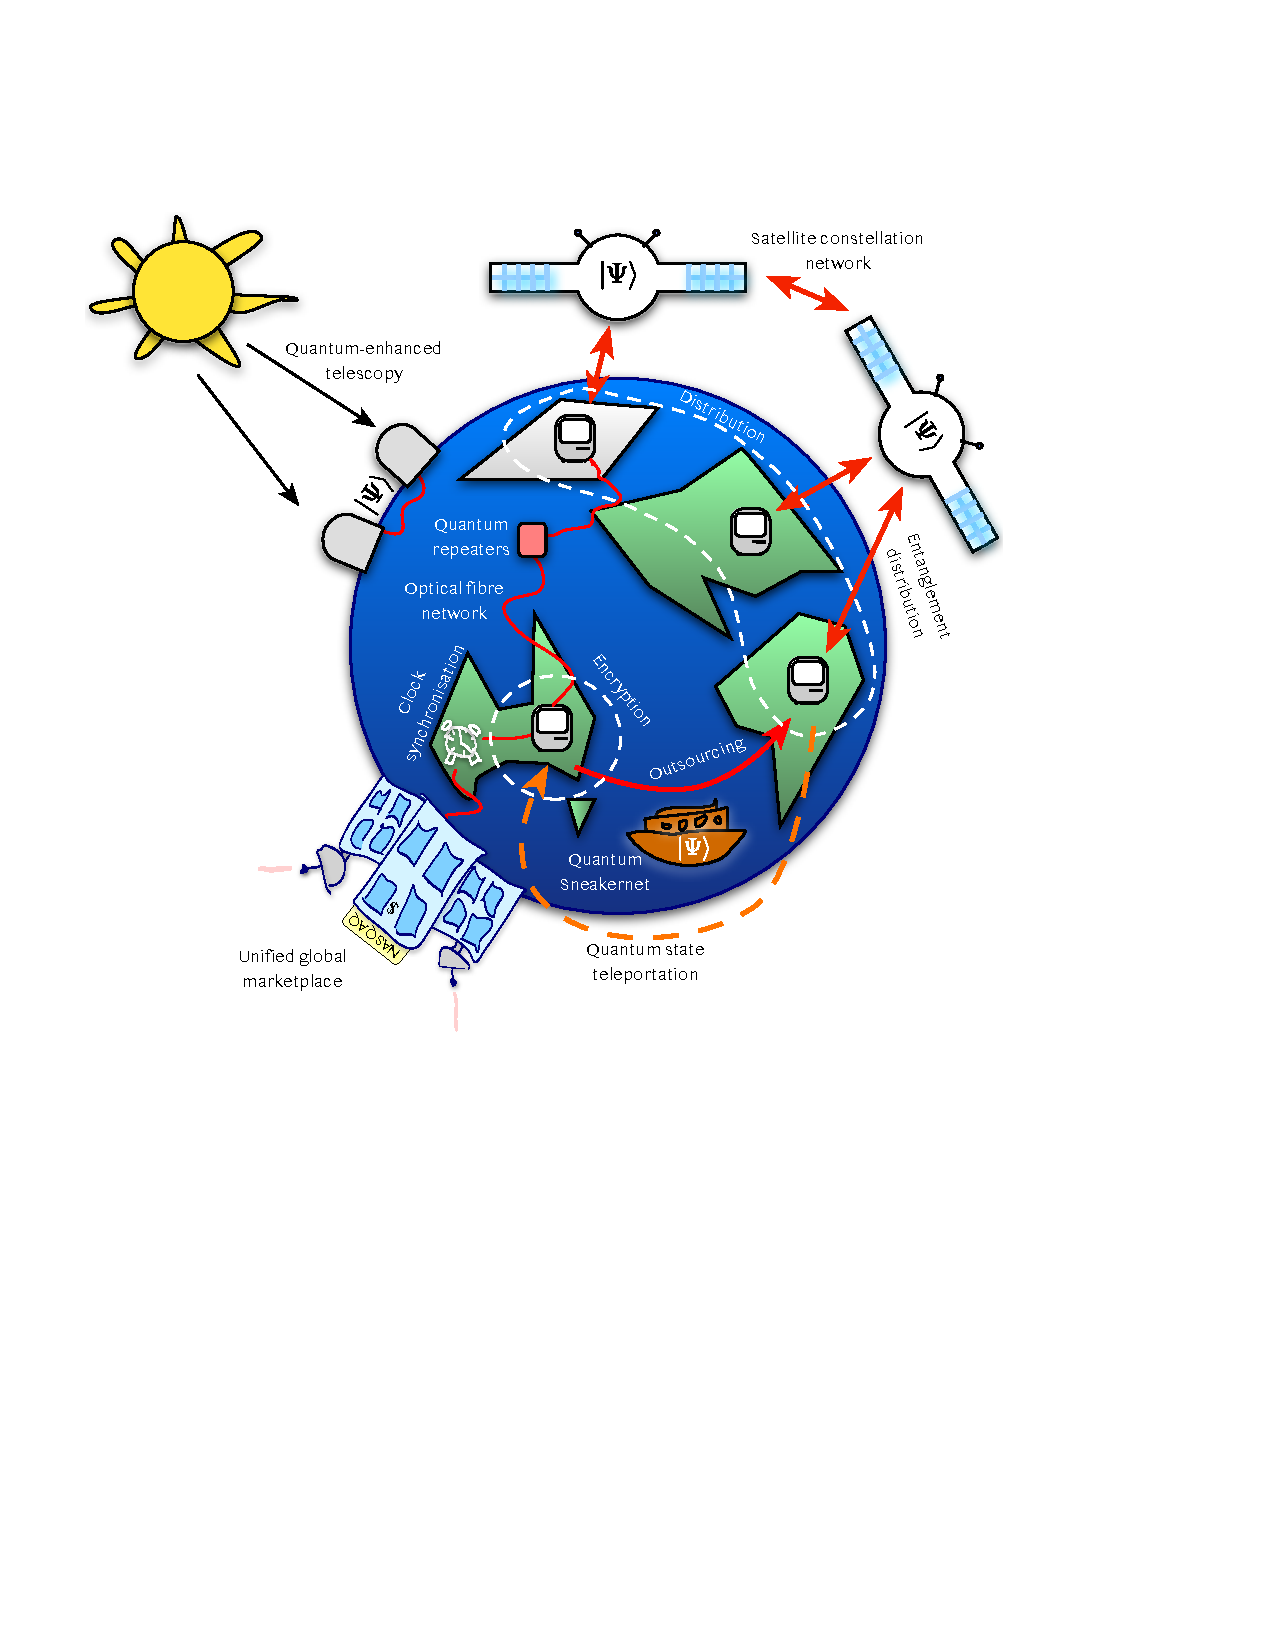
\includegraphics[clip=true, width=\textwidth]{integrated_services_overview}
	\captionspacefig \caption{Overview of some of the essential services integrated into a future globally-unified quantum internet ecosystem.}\label{fig:integrated_services_overview}
\end{figure*}